\section{Lecture 32}
\subsection{Chaos and Nonlinear Dynamics}
\subsubsection{What is chaos?}
Chaotic systems can be described as systems with extreme sensitivity to initial conditions. Nonlinearity is a necessary condition, but not sufficient (not all nonlinear systems are chaotic). 

\subsubsection{Driven Damped Pendulum}
We recall the setup of the driven damped pendulum:
\begin{center}
    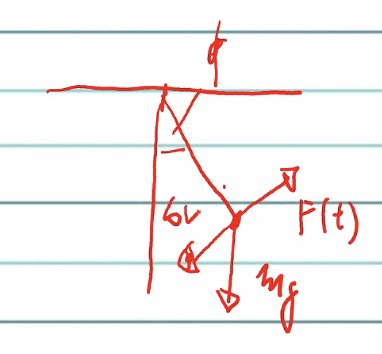
\includegraphics[scale=0.7]{Lecture-32/l32-img1.png}
\end{center}
This has the equation of motion:
\[mL^2\ddot{\phi} = -bL^2\dot{\phi} - mgL\sin\phi + LF(t)\]
Where $F(t) = F_0\cos(\omega t)$. Our standard technique for this course has been to linearize the equation, but here we want to look at the full behavior. This is where numerical simulations can come in useful. Rewriting this equation of motion slightly, we have:
\[\ddot{\phi} = -\frac{b}{m}\dot{\phi} - \frac{g}{L}\sin\phi + \frac{F_0}{mL}\cos(\omega t)\]
Define the damping parameter $2\beta = \frac{b}{m}$, the natural frequency $\omega_0^2 = \frac{g}{L}$, and the driving force $\gamma = \frac{F_0}{mL\omega_0^2}$. This yields the equation:
\[\ddot{\phi} + 2\beta\dot{\phi} + \omega_0\sin\phi = \gamma \omega_0^2\cos(\omega t)\]
Our analytical analysis of this equation ends here (as it is nonlinear), so we turn to simulations to study the behavior. 

A simulation can be found here:
\begin{center}
    \texttt{http://galileoandeinstein.physics.virginia.edu/more\textunderscore stuff/Applets/DampedDrivenPendulum/dampdrivPend\textunderscore\textunderscore1.html}
\end{center}

For a driving strength of $0.9$, looking at $\phi$ it looks quite smooth/sinusoidal. However, looking at $\dot{\phi}$, the graph is no longer sinusoidal, but quite spiky (sawtooth). Since the system is chaotic, the solutions are not just simple sine functions. Let's then move to a stronger driving of 1.05. Then, we see an initial very strange jump in the motion, before the pendulum reaches a steady state. As we drive more strongly, there is an initial transience, which eventually settles to more regular looking periodic motion.
\begin{center}
    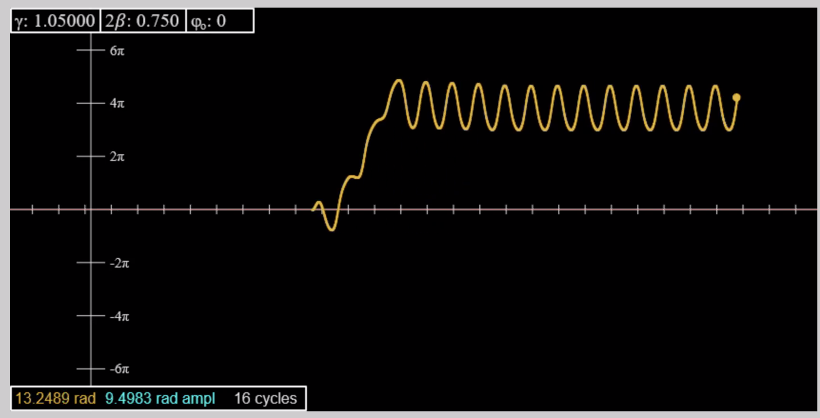
\includegraphics[scale=0.5]{Lecture-32/l32-img2.png}
\end{center}
Increasing the driving to 1.06, we see that the transient period increases even further:
\begin{center}
    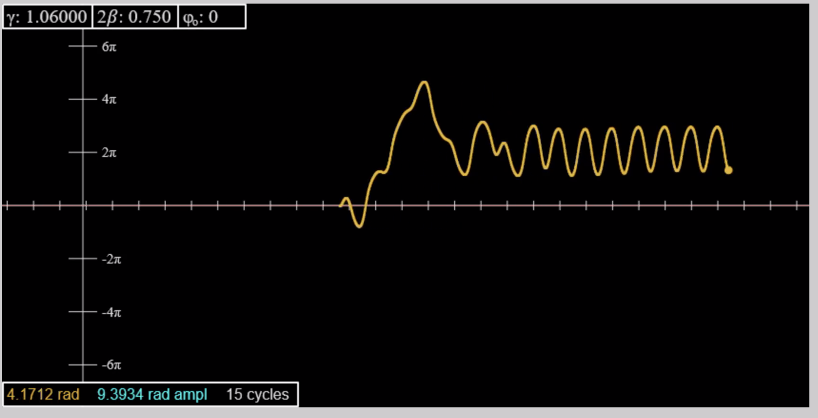
\includegraphics[scale=0.5]{Lecture-32/l32-img3.png}
\end{center}
Further increasing it to 1.07, this transient period continues to increase. If one follows the values of the high/low amplitudes (or by tracking the red line of fixed amplitude, we notice that they do not immediately repeat: 
\begin{center}
    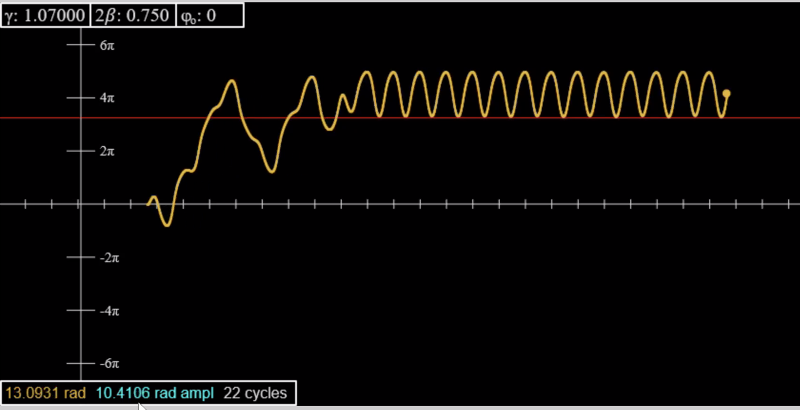
\includegraphics[scale=0.5]{Lecture-32/l32-img4.png}
\end{center}
In particular, we can see that the period doubles; period doubling is a prelude to chaos. This is \textbf{not} higher harmonics, but rather subharmonics.
\begin{center}
    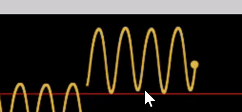
\includegraphics[scale=1]{Lecture-32/l32-img5.png}
\end{center}
Going further to a driving strength of 1.077, the motion really does not look particularly sinusoidal any longer (the strange looking motion we noticed in the transient part for weaker strengths keeps going). But by changing the initial condition, the motion changes drastically:
\begin{center}
    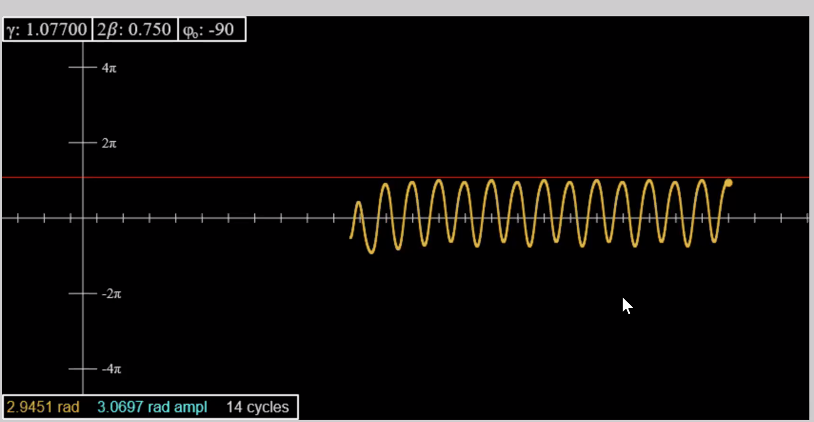
\includegraphics[scale=0.5]{Lecture-32/l32-img6.png}
\end{center}
Now, we increase the playing time and fast forward the system, to see when the transients die out, and we get a sequence of period doubling:
\begin{center}
    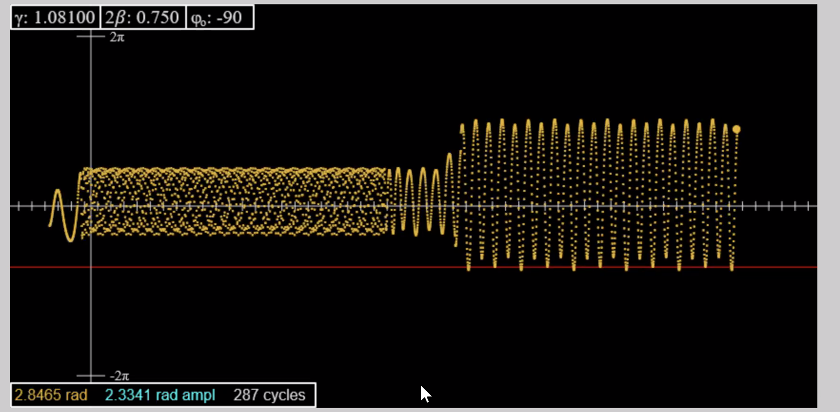
\includegraphics[scale=0.5]{Lecture-32/l32-img7.png}
\end{center}
We could also drive the pendulum very hard (1.4) and we see that hte pendulum goes wild; it swings over the top frequently. But, the motion becomes periodic; we dont see the period doubling phenomena:
\begin{center}
    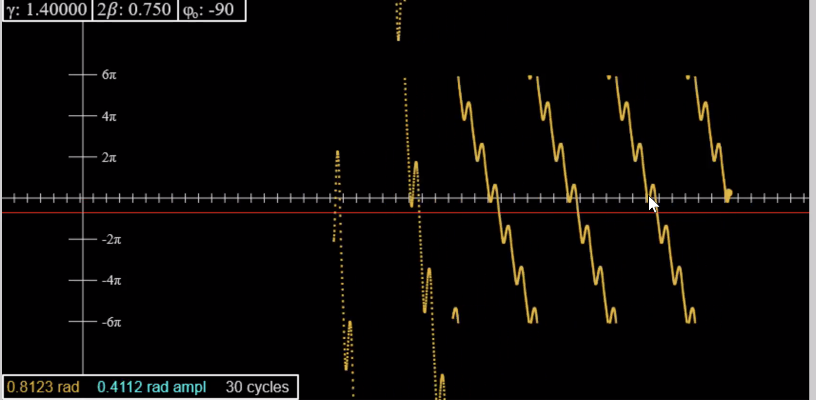
\includegraphics[scale=0.5]{Lecture-32/l32-img8.png}
\end{center}
Note that in general, chaos is not random (all of this has been deterministic), it just never repeats.

\subsubsection{Period Doubling and Bifurcations}
\begin{center}
\begin{tabular}{c|c|c}
    $n$ & period & $\gamma_m$ \\ 
    \hline
    1 & 1 to 2 & 1.0663 \\
    2 & 2 to 4 & 1.0793 \\
    3 & 4 to 8 & 1.0821 \\
    3 & 8 to 16 & 1.0827 \\
\end{tabular}
\end{center}

We see the spacings between period doubling gets narrower. Note as $\gamma_m \rightarrow \gamma_l = 1.0829$, we have chaos.

Note that this relates to a constant;
\[\gamma_{n+1} - \gamma_n = \frac{1}{\delta}(\gamma_n - \gamma_{n-1})\]
And taking $n \rightarrow \infty$ we have:
\[\delta = 4.6692016\]
Which is Feigenbaum's number. This is a unviersal constant for chaotic systems. We will explore chaos in further detail Friday.